\section{ \bfseries Linear Program (LP)}
In this problem, a linear program in the form (assume that $A$ has full column rank) is considered.\\
\begin{align*}
&\min_{x} \quad \phi=g^{\prime} x \tag{4}\label{con:op4.1}\\
& s.t. \quad A^{\prime} x=b\\
& \quad \quad  l\le x \le u
\end{align*}
%%%%%%%%%%%%%%%%%%%%%%%%%%%%%%%%%%%%%%%%%%
%%%%%%%%%%%%%%%%%%%%%%%%%%%%%%%%%%%%%%%%%%%%%%%%%%%%%%%%%%%%%%%%%%%%%%%%%%%%%%%%%%%%%
%%%%%%%%%%%%%%%%%%%%%%%%%%%%%%%%%%%%%%%%%%%
%%%%%%%%%%%%%%%%%%%%%%%%%%%%%%%%%%%%%%%%%%
%%%%%%%%%%%%%%%%%%%%%%%%%%%%%%%%%%%%%%%%%%%
\subsection{\bfseries Lagrangian function}
\begin{shaded}
{ Question: What is the Lagrangian function for this problem?}
\end{shaded}
The linear program problem (\ref{con:op4.1}) are usually stated and analyzed in the standard form, the inequlity constraints can be converted to equalities by introducing a vector of slack variables $z$ and writing

\begin{align*}
&\min_{x} \quad \phi=g^{\prime} x \tag{4.1}\\
& s.t. \quad A^{\prime} x=b\\
& \quad \quad  c(x)=\begin{bmatrix}
x-l \\ u-x\end{bmatrix}=\left[I\quad -I\right]^{\prime}x+\begin{bmatrix}
-l \\ u\end{bmatrix}\ge 0\Leftrightarrow C^{\prime}x \ge d\Leftrightarrow C^{\prime}x-z=d(z\ge 0)
\end{align*}\\[0.3cm]

The equality constraints in linear programming is always treated as $x \ge 0$ and the lagrange multipliers $\lambda$ and $s$ are introduced.The Lagrangian function is\\
$$L(x,\lambda,s)=g^{\prime}x-\lambda^{\prime}\left(A^{\prime}x-b\right)-s^{\prime}x\eqno{(4.2)}$$

%%%%%%%%%%%%%%%%%%%%%%%%%%%%%%%%%%%%%%%%%%
%%%%%%%%%%%%%%%%%%%%%%%%%%%%%%%%%%%%%%%%%%%
%%%%%%%%%%%%%%%%%%%%%%%%%%%%%%%%%%%%%%%%%%
%%%%%%%%%%%%%%%%%%%%%%%%%%%%%%%%%%%%%%%%%%%
%%%%%%%%%%%%%%%%%%%%%%%%%%%%%%%%%%%%%%%%%%
%%%%%%%%%%%%%%%%%%%%%%%%%%%%%%%%%%%%%%%%%%%
\newpage
\subsection{\bfseries Optimality conditions}
\begin{shaded}
{Question: Write the nesessary and sufficient optimality conditions for this problem.}
\end{shaded}
\begin{align*}
& \nabla_{x} L\left(x,\mu,\lambda\right)=g-A\lambda-s=0\tag{4.3}\\
& \nabla_{\lambda} L\left(x,\mu,\lambda\right)=-\left(A^{\prime}x-b\right)=0\tag{4.4}\\
& \nabla_{s} L\left(x,\mu,\lambda\right)=x \ge 0\tag{4.5}\\
& s \ge 0\tag{4.6}\\
& x_is_i=0 \quad i=1,2,...,n\tag{4.7}
\end{align*}

%%%%%%%%%%%%%%%%%%%%%%%%%%%%%%%%%%%%%%%%%%
%%%%%%%%%%%%%%%%%%%%%%%%%%%%%%%%%%%%%%%%%%%
%%%%%%%%%%%%%%%%%%%%%%%%%%%%%%%%%%%%%%%%%%
%%%%%%%%%%%%%%%%%%%%%%%%%%%%%%%%%%%%%%%%%%%
%%%%%%%%%%%%%%%%%%%%%%%%%%%%%%%%%%%%%%%%%%
%%%%%%%%%%%%%%%%%%%%%%%%%%%%%%%%%%%%%%%%%%%
\subsection{\bfseries Primal-dual interior-point algorithm}
\begin{shaded}
{Question: Write pseudo-code for a primal-dual interior-point algorithm for solution of this
problem. Explain each major step in your algorithm.}
\end{shaded}

{\setmainfont{Times New Roman}\bfseries Pseudo-code}
\begin{algorithm}[!h]
	\caption{Primal-Dual Predictor-Corrector Interior-Point Algorithm}
	\begin{algorithmic}[1]
	    \STATE Given an input $H$, $g$, $A$, $b$, and compute the starting point $x_0$, $\lambda_0$, $s_0$ with ($x_0$,$s_0$)>0\\
        \WHILE {(not converged)}\\
		\STATE Compute the affine step direction $\Delta x^{aff}$, $\Delta \lambda^{aff}$ and $\Delta s^{aff}$\\
		\STATE Compute the affine step size\  $\alpha_{aff}^{pri}$\ and\ $\alpha_{aff}^{dual}$\\
		\STATE Compute the affine duality gap $\mu_{aff} $\\
		\STATE Compute centering parameter $\sigma=\left(\mu_{aff}/\mu\right)^3$\\
		\STATE Compute affine-centering-correction direction$(\Delta x,\Delta \lambda,\Delta s)$\\
		\STATE Compute the step size $\alpha * \eta$ and update the iteration of $x^{k+1}=x^k+\alpha_k^{pri}\Delta x$, $(\lambda^{k+1},s^{k+1})=(\lambda^k,s^k)+\alpha_k^{dual}(\Delta \lambda,\Delta s)$ and $s$ to take the actual step\\
		\STATE Check convergence conditions and stop if it converged\\
		\ENDWHILE
    \end{algorithmic}
\end{algorithm}
\newpage
In the first step, a set of feasible starting point needs to be computed. A heuristic for starting point on p.410 in Nocedal \& Wright is introduced\\[0.3cm]
The problems is solved 
\begin{align*}
&\min _{x} \quad\frac{1}{2} x^{\prime} x  \qquad s.t. \quad A^{\prime}x=b \tag{4.8}\\
&\min _{(\lambda, s)} \quad\frac{1}{2} s^{\prime} s \qquad  s.t. \quad  A \lambda+s=g\tag{4.9}
\end{align*}
$\tilde{x}$, $\tilde{\lambda}$ and $\tilde{s}$ can be written as
$$\tilde{x}=A\left(A^{\prime} A\right)^{-1} b \quad \tilde{\lambda}=\left(A^{\prime} A\right)^{-1} A^{\prime} g, \quad \tilde{s}=g-A \tilde{\lambda}\eqno{(4.10)}$$
Because $\tilde{x}$ and $\tilde{s}$ should be greater than $0$
$$\delta_{x}=\max \left(-(3 / 2) \min _{i} \tilde{x}_{i}, 0\right), \delta_{s}=\max \left(-(3 / 2) \min _{i} \tilde{s}_{i}, 0\right)\eqno{(4.11)}$$
$$\hat{x}=\tilde{x}+\delta_{x} e \quad \hat{s}=\tilde{s}+\delta_{s} e \quad e=(1, \ldots, 1)^{T}$$
To ensure that the components $x^0$ and $s^0$ is not to0 close to zero or too dissimilar, two more scalars are added
$$\hat{\delta}_{x}=\frac{1}{2} \frac{\hat{x}^{T} \hat{s}}{e^{T} \hat{s}}, \quad \hat{\delta}_{s}=\frac{1}{2} \frac{\hat{x}^{T} \hat{s}}{e^{T} \hat{x}}\eqno{(4.12)}$$
$$x^{0}=\hat{x}+\hat{\delta}_{x} e, \quad \lambda^{0}=\tilde{\lambda}, \quad s^{0}=\hat{s}+\hat{\delta}_{s} e$$
The spirit of the Primal-dual interior-point algorithm for linear programming is similar to the ones for quadratic Programming, and the specific calculation process is as follows.\\[0.3cm]
First the optimal conditions
$$F(x, \lambda, s)=\left[\begin{array}{c}
A \lambda+s-g \\
A^{\prime} x-b \\
X S e
\end{array}\right]=0\eqno{(4.13)}$$
Where
$$X=\operatorname{diag}\left(x_{1}, \ldots, x_{n}\right),\quad S=\operatorname{diag}\left(s_{1}, \ldots, s_{n}\right)$$
The affine step direction is solved by
$$\left[\begin{array}{lll}
0 & A & I \\
A^{\prime} & 0 & 0 \\
S & 0 & X
\end{array}\right]\left[\begin{array}{l}
\Delta x^{\mathrm{aff}} \\
\Delta \lambda^{\mathrm{aff}} \\
\Delta s^{\mathrm{aff}}
\end{array}\right]=-\left[\begin{array}{c}
A \lambda+s-c \\
A^{\prime} x-b \\
X S e
\end{array}\right]=\left[\begin{array}{c}
-r_{c} \\
-r_{b} \\
-X S e
\end{array}\right]\eqno{(4.14)}$$
Then the affine step size can be calculated
$$\alpha_{\mathrm{aff}}^{\mathrm{pri}}=\min \left(1, \min _{i: \Delta x_{i}^{\mathrm{aff}}<0}-\frac{x_{i}}{\Delta x_{i}^{\mathrm{aff}}}\right), \quad \alpha_{\mathrm{aff}}^{\mathrm{dual}}=\min \left(1, \min _{i: \Delta s_{i}^{\mathrm{aff}}<0}-\frac{s_{i}}{\Delta s_{i}^{\mathrm{aff}}}\right)\eqno{(4.15)}$$
The Duality gap $\mu_{aff}$ is defined for affine step
$$\mu_{\mathrm{aff}}=\left(x+\alpha_{\mathrm{aff}}^{\mathrm{pri}} \delta x^{\mathrm{aff}}\right)^{T}\left(s+\alpha_{\mathrm{aff}}^{\mathrm{dual}} \delta s^{\mathrm{aff}}\right) / n\eqno{(4.16)}$$
The centering parameter
$$\sigma=\left(\frac{\mu_{\mathrm{aff}}}{\mu}\right)^{3}\eqno{(4.17)}$$
Affine-centering-correction direction is computed
$$\left[\begin{array}{ccc}
0 & A & I \\
A^{\prime} & 0 & 0 \\
S & 0 & X
\end{array}\right]\left[\begin{array}{c}
\Delta x \\
\Delta \lambda\\
\Delta s
\end{array}\right]=\left[\begin{array}{c}
-r_{c} \\
-r_{b} \\
-X S e+-\Delta X^{\mathrm{aff}} \Delta S^{\mathrm{aff}} e+\mu \sigma e
\end{array}\right]\eqno{(4.18)}$$
With the given direction, the step length can be found.\\[0.3cm]
The quantities are defined as
$$\alpha_{k, \max }^{\mathrm{pri}} \stackrel{\text { def }}{=} \min _{i: \Delta x_{i}^{k}<0}-\frac{x_{i}^{k}}{\Delta x_{i}^{k}}, \quad \alpha_{k, \max }^{\mathrm{dual}} \stackrel{\text { def }}{=} \min _{i: \Delta s_{i}^{k}<0}-\frac{s_{i}^{k}}{\Delta s_{i}^{k}}\eqno{(4.19)}$$
Then the step length 
$$\alpha_{k}^{\mathrm{pri}}=\min \left(1, \eta \alpha_{k, \max }^{\mathrm{pri}}\right), \quad \alpha_{k}^{\mathrm{dual}}=\min \left(1, \eta \alpha_{k, \max }^{\mathrm{dual}}\right)\eqno{(4.20)}$$
Finally the $x^{k+1}$, $\lambda^{k+1}$ and $s^{k+1}$ update and convergence conditions is checked and stop if it converged.



%%%%%%%%%%%%%%%%%%%%%%%%%%%%%%%%%%%%%%%%%%
%%%%%%%%%%%%%%%%%%%%%%%%%%%%%%%%%%%%%%%%%%%
%%%%%%%%%%%%%%%%%%%%%%%%%%%%%%%%%%%%%%%%%%
%%%%%%%%%%%%%%%%%%%%%%%%%%%%%%%%%%%%%%%%%%%
%%%%%%%%%%%%%%%%%%%%%%%%%%%%%%%%%%%%%%%%%%
%%%%%%%%%%%%%%%%%%%%%%%%%%%%%%%%%%%%%%%%%%%
\newpage
\subsection{\bfseries Implementation of primal-dual interior-point algorithm}
\begin{shaded}
{Question: Implement the primal-dual interior-point algorithm and test it. You must provide commented code as well as driver files to test your code, documentation that it works, and performance statistics.}
\end{shaded}
The matlab code is showed
{\setmainfont{Courier New Bold} \scriptsize            
\begin{lstlisting}
function [x,output]=ipLP(g,A,b)
% ipLP   Primal-dual interior-point algorithm
%
%          min  g'*x
%           x
%          s.t. A x  = b      
%               x >= 0      
%         rc = g − A*lambda − S = 0 
%         rb = Ax − b = 0 
%         XSe=0
%         rA = Ax + b = 0 (Lagrange multiplier y)
%         rC = Cx + s + d = 0 (Lagrange multiplier z)
%         s ≥ 0 (Slack variables )
%         sz = 0
% Syntax: [x,output]=ipLP(g,A,b)
%         output.fval: minimum value
%         output.lam : final lambda
%         output.s : final s
%         output.z: final z
%         output.Xarray: Iteration trajectory    
iteration_max=30;

epsilon=1.0e-6;
eta=0.99;
stop_flag=0;
nx=size(g,1);%x
nc=size(b,1);%c
%starting point
e=ones(nx,1);
x_hat=A'*inv(A*A')*b;
lam_hat=inv(A*A')*A*g;
s_hat=g-A'*lam_hat;

delta_x=max(-(3/2)*min(x_hat),0);
delta_s=max(-(3/2)*min(s_hat),0);

x_hat=x_hat+delta_x*e;
s_hat=s_hat+delta_s*e;

delta_x_hat=0.5*(x_hat'*s_hat)/(e'*s_hat);
delta_s_hat=0.5*(x_hat'*s_hat)/(e'*x_hat);

x0=x_hat+delta_x_hat*e;
lam0=lam_hat;
s0=s_hat+delta_s_hat*e;

Xarray=[];
Xarray=[Xarray x0];
%Predictor-Corrector algorithm
rc=A'*lam0+s0-g;
rb=A*x0-b;

x=x0;
lam=lam0;
s=s0;
iteration=0;
while(~stop_flag&iteration<=iteration_max)
    %solving the problem to obtain delta_x_aff,delta_lam_aff and delta_s_aff
    KKT_A=[zeros(nx,nx) A' eye(nx,nx);A zeros(nc,nc) zeros(nc,nx);diag(s) zeros(nx,nc) diag(x)];
    XSe=diag(x)*diag(s)*e;
    KKT_b=[-rc;-rb;-XSe];
    [L,D,p]=ldl(KKT_A, 'lower', 'vector');
    delta_aff=zeros(size(KKT_b,1),1);
    delta_aff(p)=L'\(D\(L\KKT_b(p)));
    delta_x_aff=delta_aff(1:nx);
    delta_lam_aff=delta_aff(nx+1:nx+nc);
    delta_s_aff=delta_aff(nx+nc+1:end);
    
    %calculate the alf_pri and alf_dual
    xi_deltax=-x./delta_x_aff;
    alf_pri=min([1;xi_deltax(delta_x_aff<0)]);
    si_deltas=-s./delta_s_aff;
    alf_dual=min([1;si_deltas(delta_s_aff<0)]);
    
    %calculate mu_aff and dual gap
    mu_aff=(x+alf_pri*delta_x_aff)'*(s+alf_dual*delta_s_aff)/nx;
    mu=(x'*s)/nx;
    %calculate centering parameter
    sigma=(mu_aff/mu)^3;
    %solving the problem to obtain delta_x_step, delta_lam_step and delta_s_step
    XSe_aff=-(diag(x)*diag(s)*e)-diag(delta_x_aff)*diag(delta_s_aff)*e+sigma*mu*e;
    KKT_b=[-rc;-rb;XSe_aff];
    delta_step=zeros(size(KKT_b,1),1);
    delta_step(p)=L'\(D\(L\KKT_b(p)));
    delta_x_step=delta_step(1:nx);
    delta_lam_step=delta_step(nx+1:nx+nc);
    delta_s_step=delta_step(nx+nc+1:end);
    
    %step length
    xk_deltaxk=-x./delta_x_step;
    alf_pri_k_max=min(xk_deltaxk(delta_x_step<0));
    alf_pri_k=min([1;eta*alf_pri_k_max]);
    
    sk_deltask=-s./delta_s_step;
    alf_dual_k_max=min(sk_deltask(delta_s_step<0));
    alf_dual_k=min([1;eta*alf_dual_k_max]);
    
    x=x+alf_pri_k*delta_x_step;
    lam=lam+alf_dual_k*delta_lam_step;
    s=s+alf_dual_k*delta_s_step;
    
    rc_norm=norm(rc,2);
    ra_norm=norm(rb,2);
    dual_gap=abs(x'*s/nx);
     %stop judge
    judge = [rc_norm;ra_norm;dual_gap];
    stop_flag = (length(judge(judge < epsilon)) == 3);
    %update rc and rb
    rc=(1-alf_dual_k)*rc;
    rb=(1-alf_pri_k)*rb;
    iteration=iteration+1;
    Xarray=[Xarray x];
end
fval=g'*x;
output.fval=fval;
output.lam=lam;
output.s=s;
output.iteration=iteration;
output.xarray=Xarray;
end
\end{lstlisting}}
In order to better test the performance of the algorithm, a test problem that can randomly generate parameters and adjust the number and size of variables is used.
\begin{align*}
&\min_{x} \quad \phi=g^{\prime} x \qquad g\in \mathbb{R}^{n \times 1} \tag{4.21}\label{con:op4.21}\\
& s.t. \quad A^{\prime}x=b \qquad \qquad \qquad A\in \mathbb{R}^{n \times m}\\
& \quad \quad  x\ge 0
\end{align*}

From the optimality conditions
\begin{align*}
&x_{i}=\left\{\begin{array}{ll}
\text { random positive number } & i=1,2, \ldots, m \\
0 & i=m+1, m+2, \ldots, n
\end{array}\right\tag{4.22}\\
& z_{i}=\left\{\begin{array}{ll}
\text { random positive number } & i=m+1, m+2, \ldots, n \\
0 & i=1,2, \ldots, m
\end{array}\right\tag{4.23}\\
& y=\text{random vector}\\
& \nabla_{x} L\left(x,y,z\right)=g-Ay-z=0 \Leftrightarrow g=Ay+z\tag{4.24}\\
& \nabla_{y} L\left(x,y,z\right)=-\left(A^{\prime}x-b\right)=0 \Leftrightarrow b=A^{\prime}x\tag{4.24}
\end{align*}
It is shown that the variable values($n$) range from 10 to 200, the curve of deviation expressed by $\left\|x^*-x_{result}\right\|_2$($x^*$ is the correct optimal solution and $x_{result}$ is the optimal solution obtained by the prim-dual interior point method), the curve of the objective function value corresponding to the $x_{*}$ and $x_{result}$ respectively, and the curve of the number of iterations. Please see the driver files in appendix.
\vspace{-0.5cm}
\begin{figure}[H]
\centering
\setlength{\abovecaptionskip}{-0.2cm} 
\setlength{\belowcaptionskip}{-0.5cm} 
\subfigure[Deviation]{
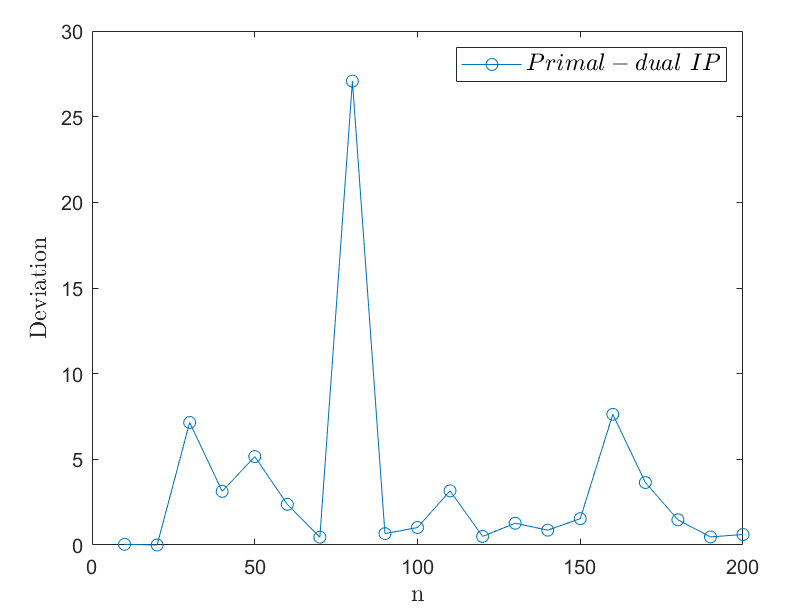
\includegraphics[scale=0.5]{figures/IP_IP_NORM.PNG}
%\caption{fig1}
}
\quad
\subfigure[Objective function value]{
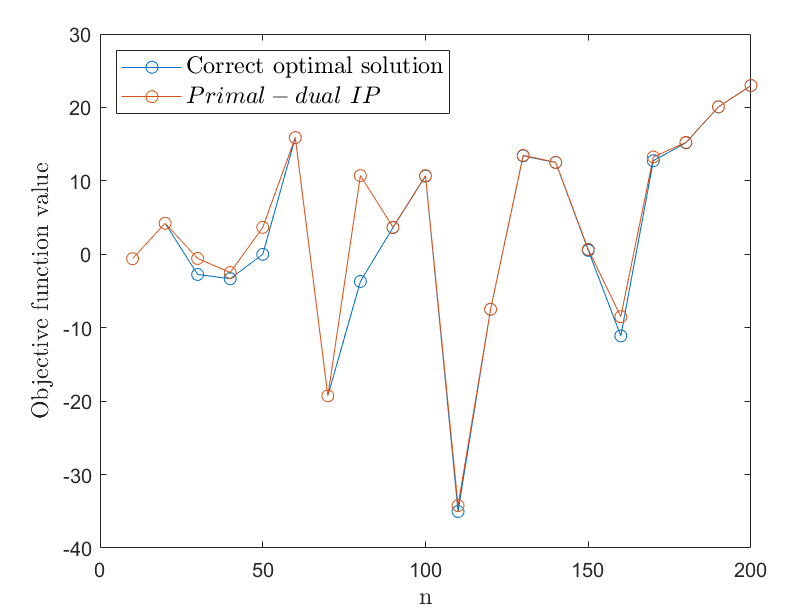
\includegraphics[scale=0.5]{figures/IP_IP_FVAL.PNG}
}
\subfigure[Iteration numbers]{
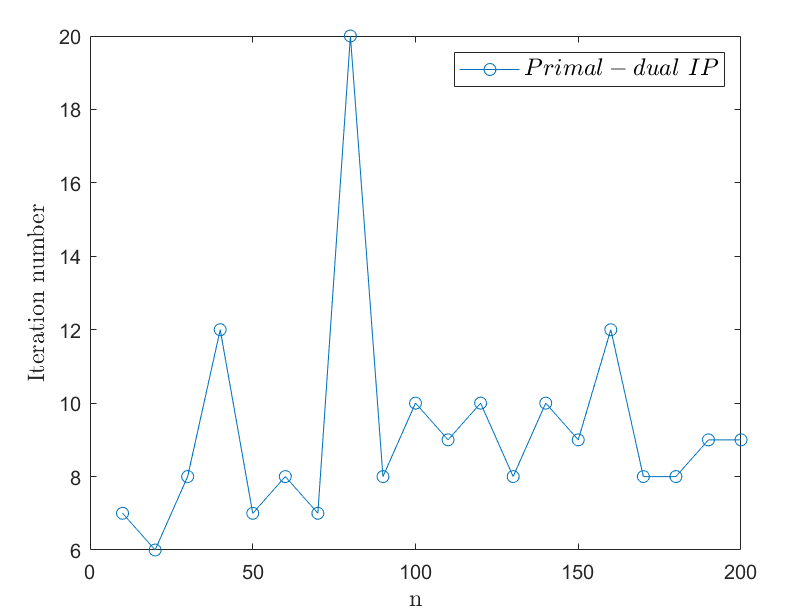
\includegraphics[scale=0.5]{figures/IP_IP_ITERATION.PNG}
}
\caption{Performance of prime-dual interior-point algorithm}
\end{figure}
It can be seen from Figures (a) and (b) that except for when the number of variables is 80($n=80$), the prime-dual interior point method can find a solution very close to the correct optimal solution. It is speculated that when the number of variables is 80, due to the randomness of the parameters in the IP problem, the interior point method encounters a singular matrix problem when solving sub-problems at certain steps, so that the correct solution cannot be obtained. According to Figure c, except for when the number of variables is 80, the prime-dual interior point method maintains a small number of iterations, and can quickly find the optimal solution.
%%%%%%%%%%%%%%%%%%%%%%%%%%%%%%%%%%%%%%%%%%
%%%%%%%%%%%%%%%%%%%%%%%%%%%%%%%%%%%%%%%%%%%
%%%%%%%%%%%%%%%%%%%%%%%%%%%%%%%%%%%%%%%%%%
%%%%%%%%%%%%%%%%%%%%%%%%%%%%%%%%%%%%%%%%%%%
%%%%%%%%%%%%%%%%%%%%%%%%%%%%%%%%%%%%%%%%%%
%%%%%%%%%%%%%%%%%%%%%%%%%%%%%%%%%%%%%%%%%%%
\subsection{\bfseries Primal simplex algorithm}
\begin{shaded}
{Question: Write pseudo-code for a primal simplex algorithm. Explain the algorithm.}
\end{shaded}
{\setmainfont{Times New Roman}\bfseries Pseudo-code}
\begin{algorithm}[!h]
	\caption{Primal simplex algorithm}
	\begin{algorithmic}[1]
	    \STATE Given a basic feasible point $x_0$ and the corresponding index set $\mathcal{B}_0$ and $\mathcal{N}_0$\\
        \WHILE {(not converged)}\\
		\STATE Solve $B^{T} \lambda=g_{B}$ for $\lambda$\\
		\STATE Compute $s_{\mathrm{N}}=g_{\mathrm{N}}-N^{T} \lambda$(pricing)\\
		\IF{($s_N \ge 0$)}\\
		\STATE Stop(optimal point found)\\
		\ENDIF\\
		\STATE Select $q \in \mathcal{N}$ with $s_{q}<0$ as the entering index;\\
		\STATE Solve $B d=A_{q}$ for $d$\\
		\IF{($d \le 0$)}
		\STATE Stop(problem is unbounded)\\
		\ENDIF
		\STATE Calculate $x_{q}^{+}=\min _{i | d_{i}>0}\left(x_{\mathrm{B}}\right)_{i} / d_{i},$ and use $p$ to denote the minimizing $i$\\
		\STATE Update $x_{\mathrm{B}}^{+}=x_{\mathrm{B}}-d x_{q}^{+}, x_{\mathrm{N}}^{+}=\left(0, \ldots, 0, x_{q}^{+}, 0, \ldots, 0\right)^{T}$\\
		\STATE Change $\mathcal{B}$ by adding $q$ and removing the basic variable corresponding to column $p$ of $B$\\
		\ENDWHILE
    \end{algorithmic}
\end{algorithm}\\


Assuming that the matrix $A$ has full column rank, each iterate generated by the simplex method is a basic feasible point of (\ref{con:op4.1}). A
vector $x$ is a basic feasible point if it is feasible and if there exists a subset $\mathcal{B}$ of the index set
$\{1, 2, . . . , n\}$, which called the basis for this problem.\\[0.3cm]
$$B=\left[A_{i}^{\prime}\right]_{i \in \mathcal{B}}\eqno{(4.25)}$$
The basic idea is to start from a vertice of the feasible , and then find the next vertice that makes the objective function smaller from the current vertice along the edge of the feasible polytope, and move to a better one if it can be found for which the basis $\mathcal{B}$ differs. However, another type
of step occurs when the problem is unbounded: The step is an edge along which the objective
function is reduced, and along which iteration point can move infinitely far without ever reaching a
vertex.
The nonbasic matrix is defined as $N=\left[A_{i}^{\prime}\right]_{i \in \mathcal{N}}$ and partition the n-element vectors $x$, $s$, and $g$
according to the index sets $\mathcal{B}$ and $\mathcal{N}$
$$\begin{array}{ll}
x_{\mathrm{B}}=\left[x_{i}\right]_{i \in \mathcal{B}}, & x_{\mathrm{N}}=\left[x_{i}\right]_{i \in \mathcal{N}} \\
s_{\mathrm{B}}=\left[s_{i}\right]_{i \in \mathcal{B}}, & s_{\mathrm{N}}=\left[s_{i}\right]_{i \in \mathcal{N}} \\
g_{\mathrm{B}}=\left[g_{i}\right]_{i \in \mathcal{B}}, & g_{\mathrm{N}}=\left[g_{i}\right]_{i \in \mathcal{N}}
\end{array}$$
From the KKT condition
$$A^{\prime} x=B x_{\mathrm{B}}+N x_{\mathrm{N}}=b\eqno{(4.26)}$$
The primal variable $x$ for this simplex iterate is defined as
$$x_{\mathrm{B}}=B^{-1}b, \qquad x_{\mathrm{N}=0}$$
In order to satisfy the complementarity condition $x_is_i=0$, $ s_{B}=0$ is defined. The remaining components $\lambda$ and $s_N$ can be found by partitioning this condition into $g_B$ and $g_N$
components and using $ s_{B}=0$  to obtain
$$B^{T} \lambda=g_{\mathrm{B}}, \quad N^{T} \lambda+s_{\mathrm{N}}=g_{\mathrm{N}}\eqno{(4.27)}$$
$s_{N}$ can be expressed by $\lambda$
$$s_{\mathrm{N}}=c_{\mathrm{N}}-N^{T} \lambda=c_{\mathrm{N}}-\left(B^{-1} N\right)^{T} c_{\mathrm{B}}\eqno{(4.28)}$$
In order to satisfy the non-negativity of condition$s\ge 0$, To be sure that the $s_B$ certainly satisfy this condition, so if $s_N\ge 0$, an optimal solution can be found. However, there are always one or more of the components of $s_N$ are negative. Then the new index which is one of the indices $q\in \mathcal{N}$ for which $s_q<0$ needs to be chose to enter the basis $\mathcal{B}$. It is called as "entering index"\\[0.3cm]
This process of selecting entering and leaving indices, and performing the algebraic
operations necessary to keep track of the values of the variables $x$, $\lambda$, and $s$, is sometimes
known as pivoting
Then the new iterate $x_B$ updates
$$x_{\mathrm{B}}^{+}=x_{\mathrm{B}}-B^{-1} A_{q}^{\prime} x_{q}^{+}\eqno{(4.29)}$$
It is found that if $d=B^{-1} A_{q}^{\prime}\le 0$, $x_{q}^{+}$ can increase to $\propto$ without ever encountering a new vertex. When this happens, the linear program is unbounded

%%%%%%%%%%%%%%%%%%%%%%%%%%%%%%%%%%%%%%%%%%
%%%%%%%%%%%%%%%%%%%%%%%%%%%%%%%%%%%%%%%%%%%
%%%%%%%%%%%%%%%%%%%%%%%%%%%%%%%%%%%%%%%%%%
%%%%%%%%%%%%%%%%%%%%%%%%%%%%%%%%%%%%%%%%%%%
%%%%%%%%%%%%%%%%%%%%%%%%%%%%%%%%%%%%%%%%%%
%%%%%%%%%%%%%%%%%%%%%%%%%%%%%%%%%%%%%%%%%%%
\subsection{\bfseries Implementation of primal simplex algorithm}
\begin{shaded}
{Question: Implement a primal active-set algorithm (a primal simplex algorithm) for the
linear program. You must provide commented code as well as driver files to
test your code, documentation that it works, and performance statistics.}
\end{shaded}
{\setmainfont{Courier New Bold} \scriptsize            
\begin{lstlisting}
function [x,output]=Pri_Simple(c,A,b,base)
% Pri_Simple  Primal simplex algorithm
%          min  c'*x
%           x
%          s.t. A x  = b      
%               x >= 0   
%         base: base vector
% Syntax: [x,output]=Pri_Simple(c,A,b,base)
%         output.fval: minimum value
%         output.case: 
%                      'found' : optimal solution found
%                      'unbound' : the problem is unbounded
%         output.xarray: Iteration trajectory  
iteration_max=400;
iteration=0;
Xarray=[];
nx=size(A,2);
nc=size(A,1);
%if c>=0 the x can be calculated directly, but only if the constraint is satisfied
if c>=0
    index_c=find(c~=0,1,'last');
    test_c=inv(A(:,(nx-nc+1):nx))*b;
    if test_c>=0
        x=zeros(1,index_c);
        output.fval=0;
    else
        output.case='no optimal point';
        x=NaN;
        output.fval=NaN;
        return;
    end
end
%Initialization of nobasevector
nobase=zeros(1,1);
comp1=1:nx;
count=1;
for i=1:nx
    if(isempty(find(base==comp1(i),1)))
        nobase(count)=i;
        count=count+1;
    end
end
B=A(:,base);
x_B=inv(B)*b;
while(iteration<=iteration_max)
    B=A(:,base);
    N=A(:,nobase);
    c_B = c(base);
    c_N = c(nobase);
    x_B=inv(B)*b;
    
    lambda=inv(B)'*c_B;
    for i=1:length(nobase)
    s_N(i)=c_N(i)-N(:,i)'*lambda;
    end
    [min_q,index_q]=min(s_N);
    %optimal solution found
    if min_q>=0
        output.case='found';
        output.fval=c_B'*x_B;
        index_c=find(c~=0,1,'last');
        for i=1:index_c
            value_c=find(base==i,1);
            if isempty(value_c)
                x(i)=0;
            else
                x(i)=x_B(value_c);
            end
        end
        break;
    end
    %current value
    index_c=find(c~=0,1,'last');
        for i=1:index_c
            value_c=find(base==i,1);
            if isempty(value_c)
                x_tmp(i)=0;
            else
                x_tmp(i)=x_B(value_c);
            end
        end
    x=x_tmp;
    %fprintf("step %d,the current feasible solution is:\n",iteration)
    %fprintf('%.4f, ',x_tmp);
    %fprintf(',\nand the value of z is %.4f\n\n',c_B'*x_B);
    %solve d
    d=inv(B)*A(:,nobase(index_q));
    
    if d<=0
        x=NaN;
        output.fval=NaN;
        output.case='unbounded';
        return;
    end
    %find the leaving indices
    min_xq=inf;
    index_xq=0;
    for i=1:length(d)
        if d(i)>0
            xq=x_B(i)/d(i);
            if xq<min_xq
                min_xq=xq;
                index_xq=i;
            end
        end
    end
    %update the basevector and nobasevector
    tmp=base(index_xq);
    base(index_xq)=nobase(index_q);
    nobase(index_q)=tmp;
    %update x_B
    x_B=x_B-d*min_xq;
    iteration=iteration+1;
    Xarray=[Xarray x_tmp];
end
output.iteration=iteration;
output.xarray=Xarray;
end
\end{lstlisting}}
The same problem is used to test primal simplex algorithm as described in section 4.4. It is shown that the variable values($n$) range from 10 to 200, the curve of deviation expressed by $\left\|x^*-x_{result}\right\|_2$($x^*$ is the correct optimal solution and $x_{result}$ is the optimal solution obtained by the primal simplex algorithm), the curve of the objective function value corresponding to the $x_{*}$ and $x_{result}$ respectively, and the curve of the number of iterations. Please see the driver files in appendix.

\begin{figure}[H]
\centering
\subfigure[Deviation]{
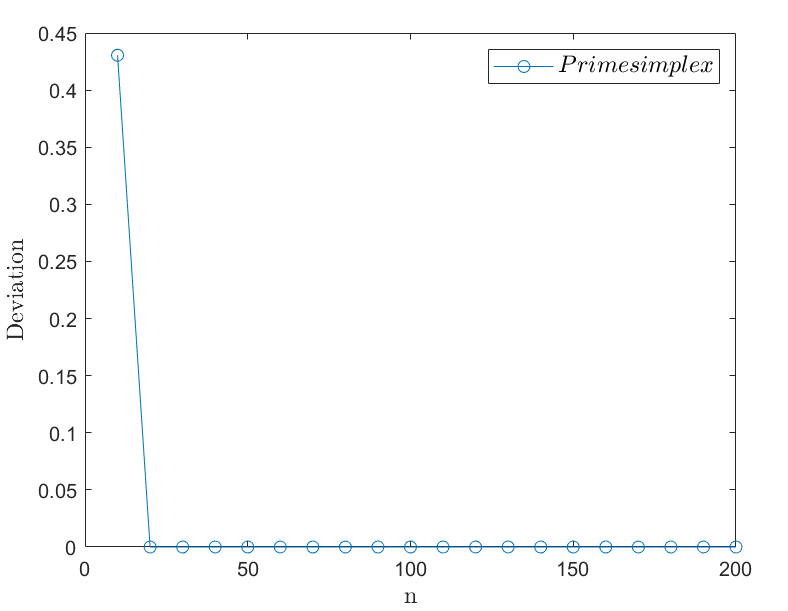
\includegraphics[scale=0.5]{figures/IP_SIMPLEX_NORM.PNG}
%\caption{fig1}
}
\quad
\subfigure[Objective function value]{
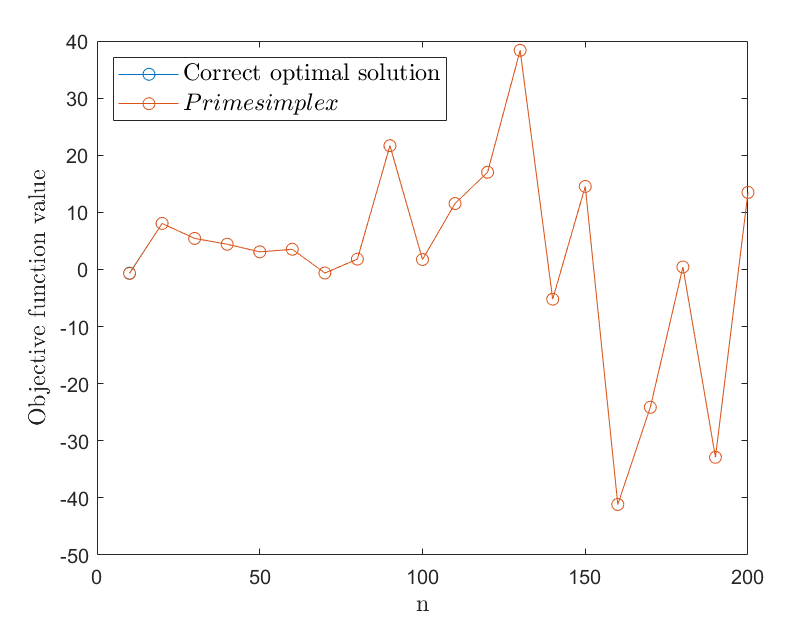
\includegraphics[scale=0.5]{figures/IP_SIMPLEX_FVAL.PNG}
}
\subfigure[Iteration numbers]{
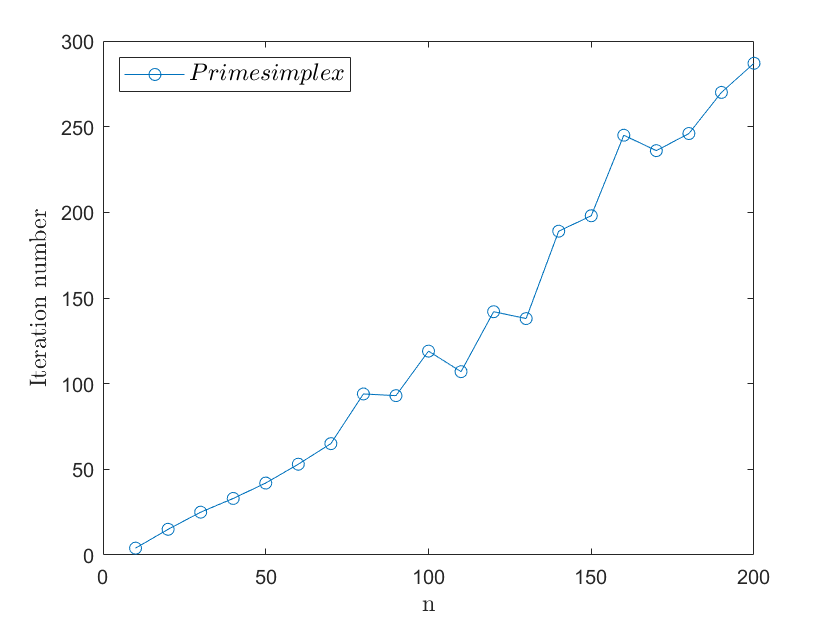
\includegraphics[scale=0.5]{figures/IP_SIMPLEX_ITERATION.PNG}
}
\caption{Performance of primal simplex algorithm}
\end{figure}
It should be noted in Figure b that the objective function value of the correct optimal solution is exactly the same as the value of the optimal value obtained by the simplex method. That is why there is only one curve in figures b. As can be seen from figures a and b, no matter how the number of variables Changes, the simplex method can always find the optimal solution, but at the same time can be seen from Figure c, the number of iterations of the simplex method is gradually increasing.
%%%%%%%%%%%%%%%%%%%%%%%%%%%%%%%%%%%%%%%%%%%%%%%%%%%%%%%%%%%%%%%%%%%%%%%%%%%%%%%%%%%%%%%%%%%%%%%%%%%%%%%%%%%%%%%%%%%%%%%%%%%%%%%%%%%%%%%%%%%%%%%%%%%%%%%%%%%%%%%%%%%%%%%%%%%%%%%%%%%%%%%%%%%%%%%%%%%%%%%%%%%%%%%%%%%%%%%%%%%%%%%%%%%%%%%%%%%%%%%%%%%%%%%%%%%%%%%%%%%%%%%%%%%%%%%%%%%%%%%%%%%%%%%%%%%%%%%%%%%%%%%%%%%%%%%%%%%%%%%%%%%%%%%%%%%%%%%%%%%%%%%%%%%%%%%%%%%%%%%%%%%%%%%%%%%%%%%%%%%%%%%%%%%%%%%%%%%%%%%%%%%%%%%%%%%%%%%%%%%%%%%%%%%%%%%%%%%%%%%%%%%%%%%%%%%%%%%%%%%%%%%%%%%%%%%%%%%%%%%%%%%%%%%%%%%%
\newpage
\subsection{\bfseries Comparison of algorithms}
\begin{shaded}
{Question: Compare the performance of your primal-dual interior-point algorithm, primal
active-set algorithm (primal simplex algorithm), and linprog from Matlab (or
equivalent LP library functions). Provide scripts that demonstrate how you compare the software and comment on the tests and the results.}
\end{shaded}
The same problem is used to test primal simplex algorithm as described in section 4.4. The primal-dual interior-point algorithm, primal simplex algorithm, and linprog("Dual-simplex" is used here) from Matlab are tested. Please see the driver files in appendix \ref{6.4.1}. It is shown that the variable values($n$) range from 10 to 200, the curve of deviation expressed by $\left\|x^*-x_{result}\right\|_2$($x^*$ is the correct optimal solution and $x_{result}$ is the optimal solution obtained by tested three algorithms), the curve of the objective function value corresponding to the $x_{*}$ and $x_{result}$ respectively, and the curve of the number of iterations.
\vspace{-0.5cm}
\begin{figure}[H]
\centering
\setlength{\abovecaptionskip}{-0.2cm} 
\setlength{\belowcaptionskip}{-0.5cm} 
\subfigure[Deviation]{
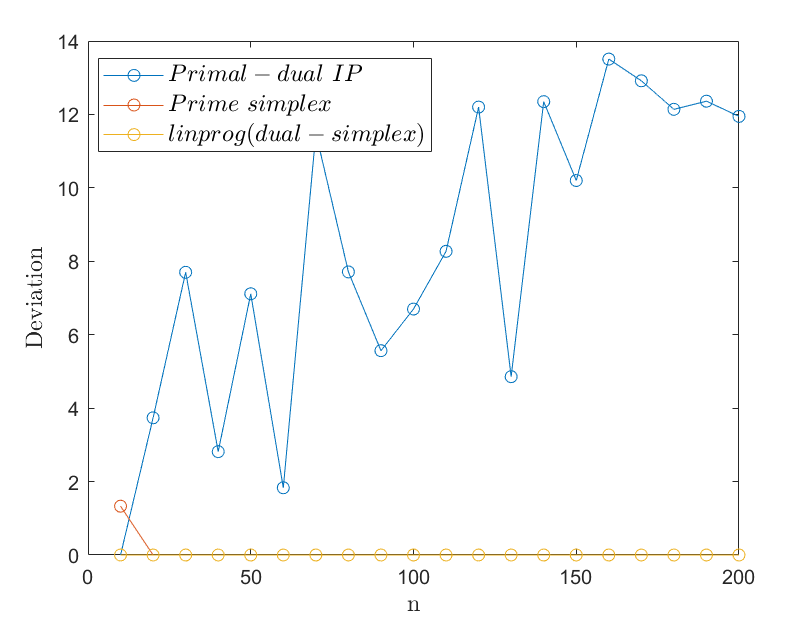
\includegraphics[scale=0.5]{figures/IP_NORM.PNG}
%\caption{fig1}
}
\quad
\subfigure[Objective function value]{
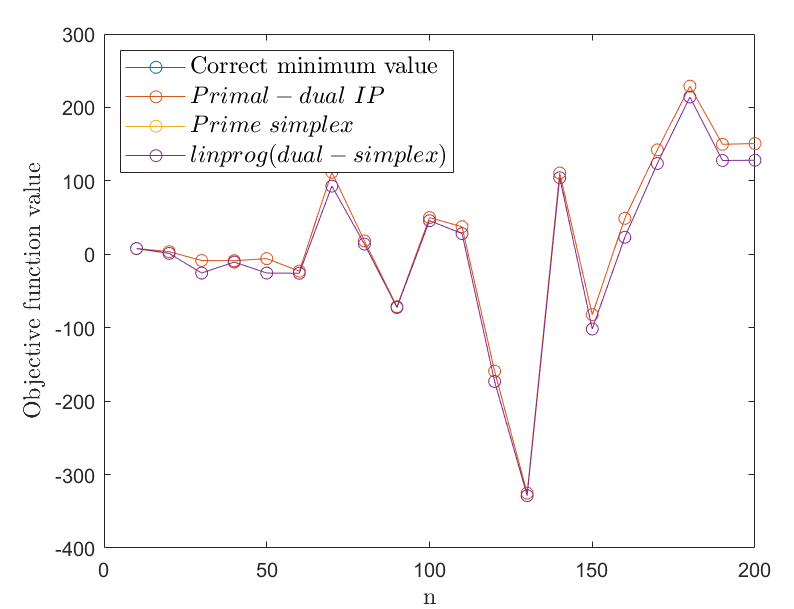
\includegraphics[scale=0.5]{figures/IP_FVAL.PNG}
}
\subfigure[Iteration numbers]{
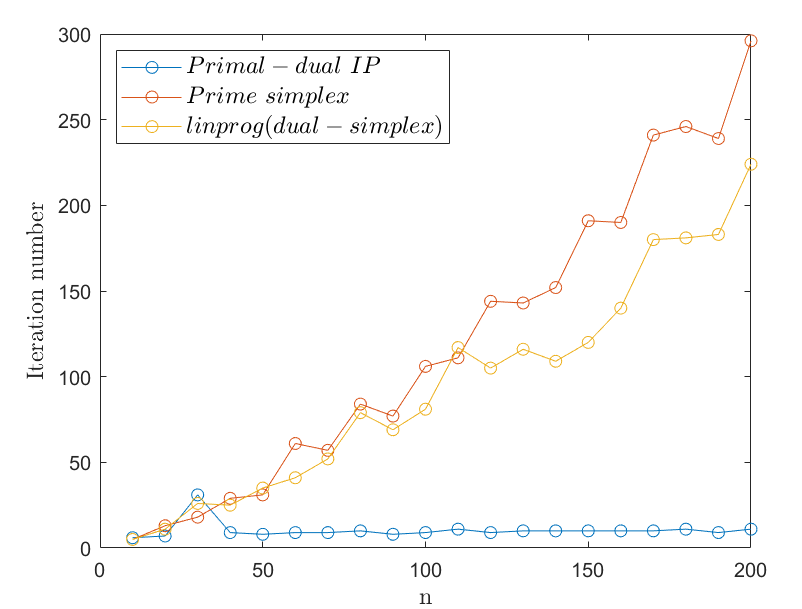
\includegraphics[scale=0.5]{figures/IP_ITERATION.PNG}
}
\caption{Performance of the primal-dual interior-point algorithm, primal simplex algorithm, and linprog("Dual-simplex")}
\end{figure}

Through Figure a, it is found that the test results are consistent with the characteristics of the prime dual interior point method and the simplex method. With the increase in the number of variables, although the interior point method can also approach the correct optimal function, the deviation of the correct optimal solution and found optimal solution will increase larger, but both the prime simplex method implemented and the linprog's dual simplex method can always find the correct optimal solution. This feature can also be verified in Figure b. However, through Figure (c) it can be found that the simplex method can always find the optimal solution at the cost of increasing the number of iterations, which takes more time. The prime-dual interior point method can ensure that the optimal solution can be found in a small number of iterations no matter how many variables are increased.
%%%%%%%%%%%%%%%%%%%%%%%%%%%%%%%%%%%%%%%%%%%%%%%%%%%%%%%%%%%%%%%%%%%%%%%%%%%%%%%%%%%%%%%%%%%%%%%%%%%%%%%%%%%%%%%%%%%%%%%%%%%%%%%%%%%%%%%%%%%%%%%%%%%%%%%%%%%%%%%%%%%%%%%%%%%%%%%%%%%%%%%%%%%%%%%%%%%%%%%%%%%%%%%%%%%%%%%%%%%%%%%%%%%%%%%%%%%%%%%%%%%%%%%%%%%%%%%%%%%%%%%%
 \subsection{\bfseries Markowitz’ portfolio optimization problem as IP}
\begin{shaded}
{Question: Test this on a special Markowitz portfolio optimization problem where we do not
care about risk but just want to maximize the return. Formulate this Markowitz
portfolio optimization problem and test your algorithms. Discuss your tests and
the results. You should solve the problem using your primal-dual interior-point
algorithm, your primal active-set algorithm, and a library algorithm e.g. linprog}
\end{shaded}
Consider a financial market with 5 securities.\\[0.3cm]
\begin{tabular}{c|ccccc|c}
\hline Security & \multicolumn{5}{|c|} { Covariance } &  Return\\
\hline 1 & 2.30 & 0.93 & 0.62 & 0.74 & -0.23 & 15.10 \\
2 & 0.93 & 1.40 & 0.22 & 0.56 & 0.26 & 12.50 \\
3 & 0.62 & 0.22 & 1.80 & 0.78 & -0.27 & 14.70 \\
4 & 0.74 & 0.56 & 0.78 & 3.40 & -0.56 & 9.02 \\
5 & -0.23 & 0.26 & -0.27 & -0.56 & 2.60 & 17.68 \\
\hline
\end{tabular}\\[0.3cm]
The risk is not cared about, so the Linear programming form of Markowitz’ portfolio optimization problem is
\begin{align*}
&\max_{x \in \mathbb{R}^{n}} \quad \phi=x^{\prime} \mu \tag{4.30}\\
& s.t. \quad \sum_{i=1}^{n} x_{i}=1\\
& \quad \quad \ x \ge 0
\end{align*}
Then a portfolio will be computed to obtain maximum of return and the optimal
portfolio, by the primal-dual interior-point algorithm, primal simplex algorithm, and linprog("Dual-simplex" is used here) from Matlab. Please see the driver files in appendix. The result and the iteration numbers are showed\\
The primal-dual interior-point QP algorithm
\begin{align*}
&    x=(0,0,0,0,1)^{\prime}\\
&Return: \quad E\{ R\}=17.68\\
&Iteration=4
\end{align*}
The
primal simplex algorithm
\begin{align*}
&    x=(0,0,0,0,1)^{\prime}\\
&Return: \quad E\{ R\}=17.68\\
&Iteration=1
\end{align*}
The "linprog" with "Dual-simplex"
\begin{align*}
&    x=(0,0,0,0,1)^{\prime}\\
&Return: \quad E\{ R\}=17.68\\
&Iteration=1
\end{align*}
From the same results obtained from the three algorithms, it can be concluded that when risk is not considered, this Markowitz’ portfolio optimization problem can be transformed into a standard linear programming problem only for maximizing returns. The iteration point will eventually iterate to the vertex with the highest return, that is, the fifth security has the highest return of 17.68. At the same time, it is found that in the case where the minimum point is at the constrained vertex, the simplex method finds the optimal value in only one iteration with the help of the movement at the constrained boundary. Although the prime dual interior point method can also approach the minimum point, it requires an additional number of iterations compared to the simplex method.